%\documentclass[a4paper]{article}
%\usepackage[letterpaper,top=2.5cm,bottom=2cm,left=3cm,right=3cm,marginparwidth=1.75cm]{geometry}

%\documentclass[a4paper,12pt]{memoir}

\documentclass[a4paper,12pt]{article}
\usepackage[letterpaper,top=2.5cm,bottom=3cm,left=3cm,right=3cm,marginparwidth=1.75cm]{geometry}
\linespread{1.5}

\usepackage{graphicx}

\title{February status update: Echo State Networks}
\author{Hector Morlet \\ 22247737}
\date{\today}

%\chapterstyle{ger}

%\setlrmarginsandblock{4cm}{2cm}{*}
%\setulmarginsandblock{3.5cm}{3cm}{*}
%\checkandfixthelayout

\begin{document}

\maketitle

\section{Terms}

Terms we've used in the past but to be clear:
\begin{itemize}
\item "ON" is ordinal network
\item "ON ESN" refers to the layered ESN where each ordinal partition has its own layer.
\item "Stochastic ON ESN" refers to the stochastic version of the "ON ESN".
\item "Vanilla ESN" refers to an ESN without any of the layering nonsense
\end{itemize}


\section{Error fixing}

First I fixed a couple errors which we found in our last meeting, including:
For the Stochastic ON ESN, I was masking all the connections between layers other than the single randomly chosen connection only for the active layer (i.e. the layer whose partition has just been seen). I fixed it so that it chooses a connected layer for each layer according to the transition probabilities of the corresponding partitions.
For the ON ESN, there was a silly error where each node in each layer was connected to itself by a fixed amount. I removed these self-connections. But I might reintroduce them later to see what effect they have.


\section{Stochastic ON ESN: Re-scaling the reservoir weights each time the different connections are masked.}

\textbf{Background}: For each partition, the stochastic ON ESN chooses one other partition based on the transition probabilities. It then masks (sets to zero) all connections between layers, other than the chosen connections. The issue is that this means the reservoir weight matrix is constantly changing. Thus, the overall 'signal amplitude' in the network may be too low or too high. Of course, this is usually controlled by scaling the weights initially using the spectral radius.

\textbf{Hypothesis}: will rescaling the reservoir weight matrix using the spectral radius after the non-chosen weights are masked improve the prediction?

\textbf{Result}: calculating the maximum eigen value of the weight matrix each time step makes the ESN run \textit{extremely} slow. So I don't have any results. I think I will try to overcome this by caching all the possible combinations of chosen partitions and calculating the associated maximum eigenvalue for each combination. Then it won't have to calculate it each time, and probably won't need too much more memory.



\section{Testing the ON ESN using multi-step predictions.}

I can't remember why, but I stopped testing for multi-step predictions and I think my original method was producing wild results because it would feed in the partition of the true data alongside previous predictions (which would not match the partition). Now I have fixed it.

The way it now works is to run the ESN over the whole (true) time series and save the state at each time step. Then it splits the ESN into chunks and looks up the state of the ESN at the start of each chunk. Then it creates a prediction from that state and determins what the next partition is using that prediction and feeds them both back into the ESN to get the next state. It repeats this for the length of the chunk. Then the error is calculated from the predictions within each chunk over the whole series. This is what it looks like:

%\begin{figure}
%    \centering
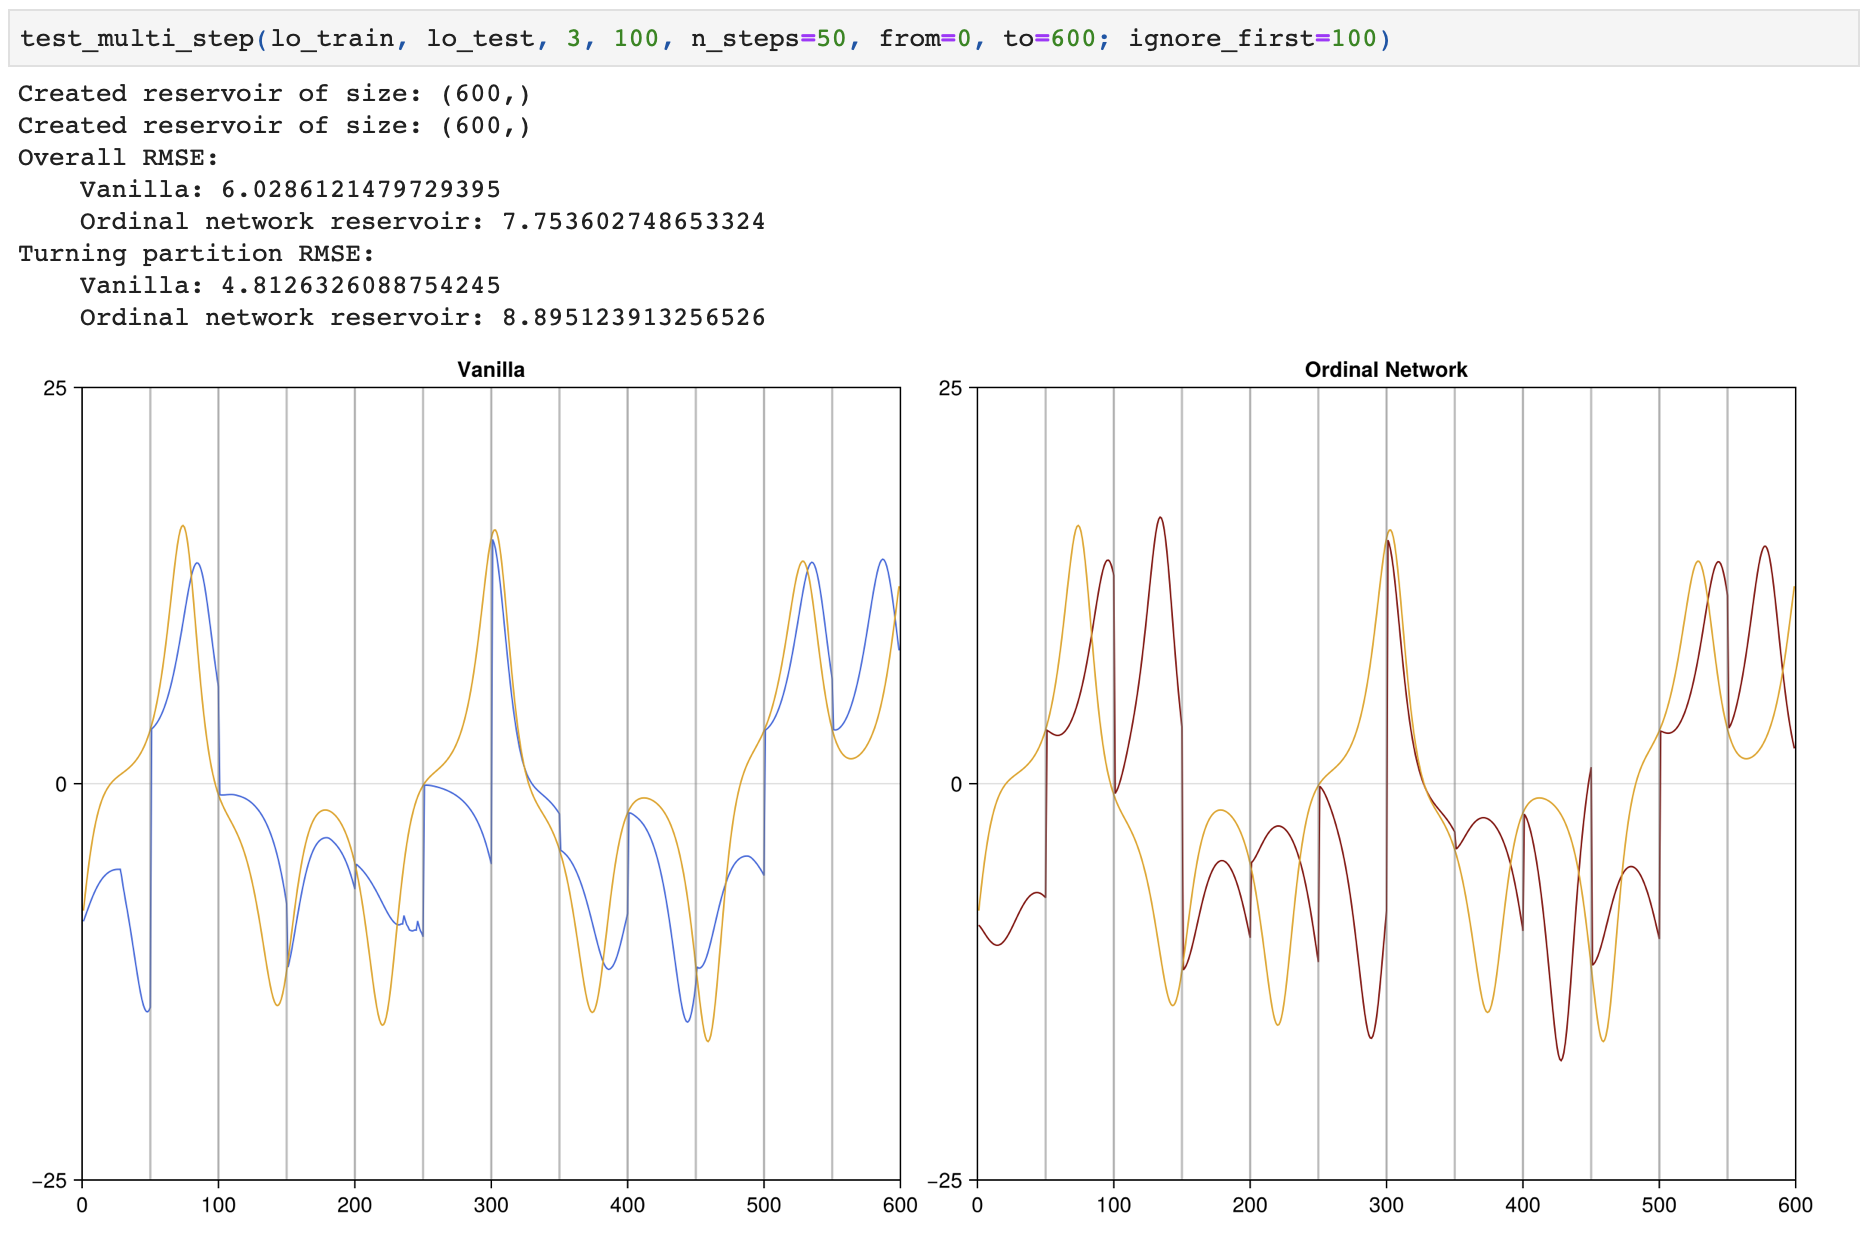
\includegraphics[width=\textwidth]{figure_1.png}
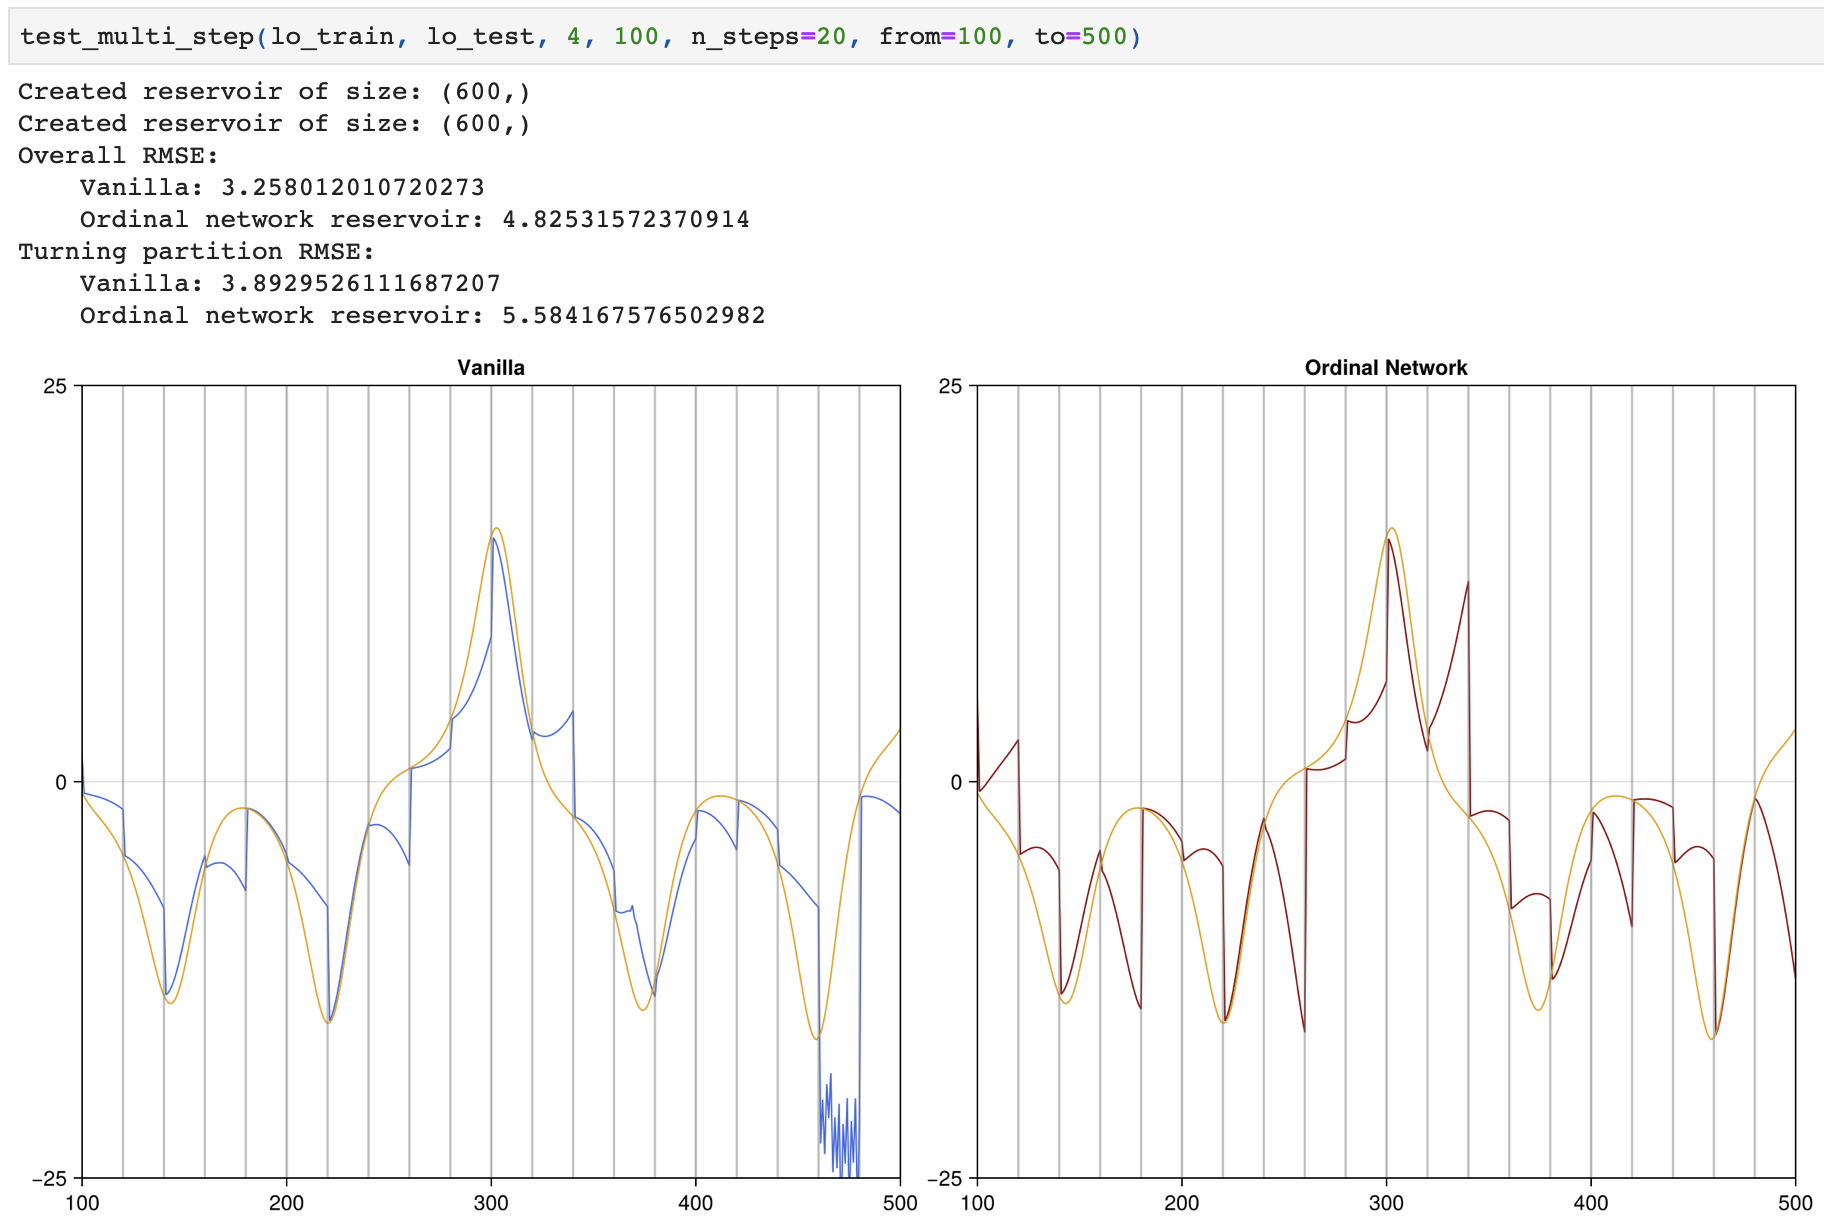
\includegraphics[width=\textwidth]{figure_2.png}
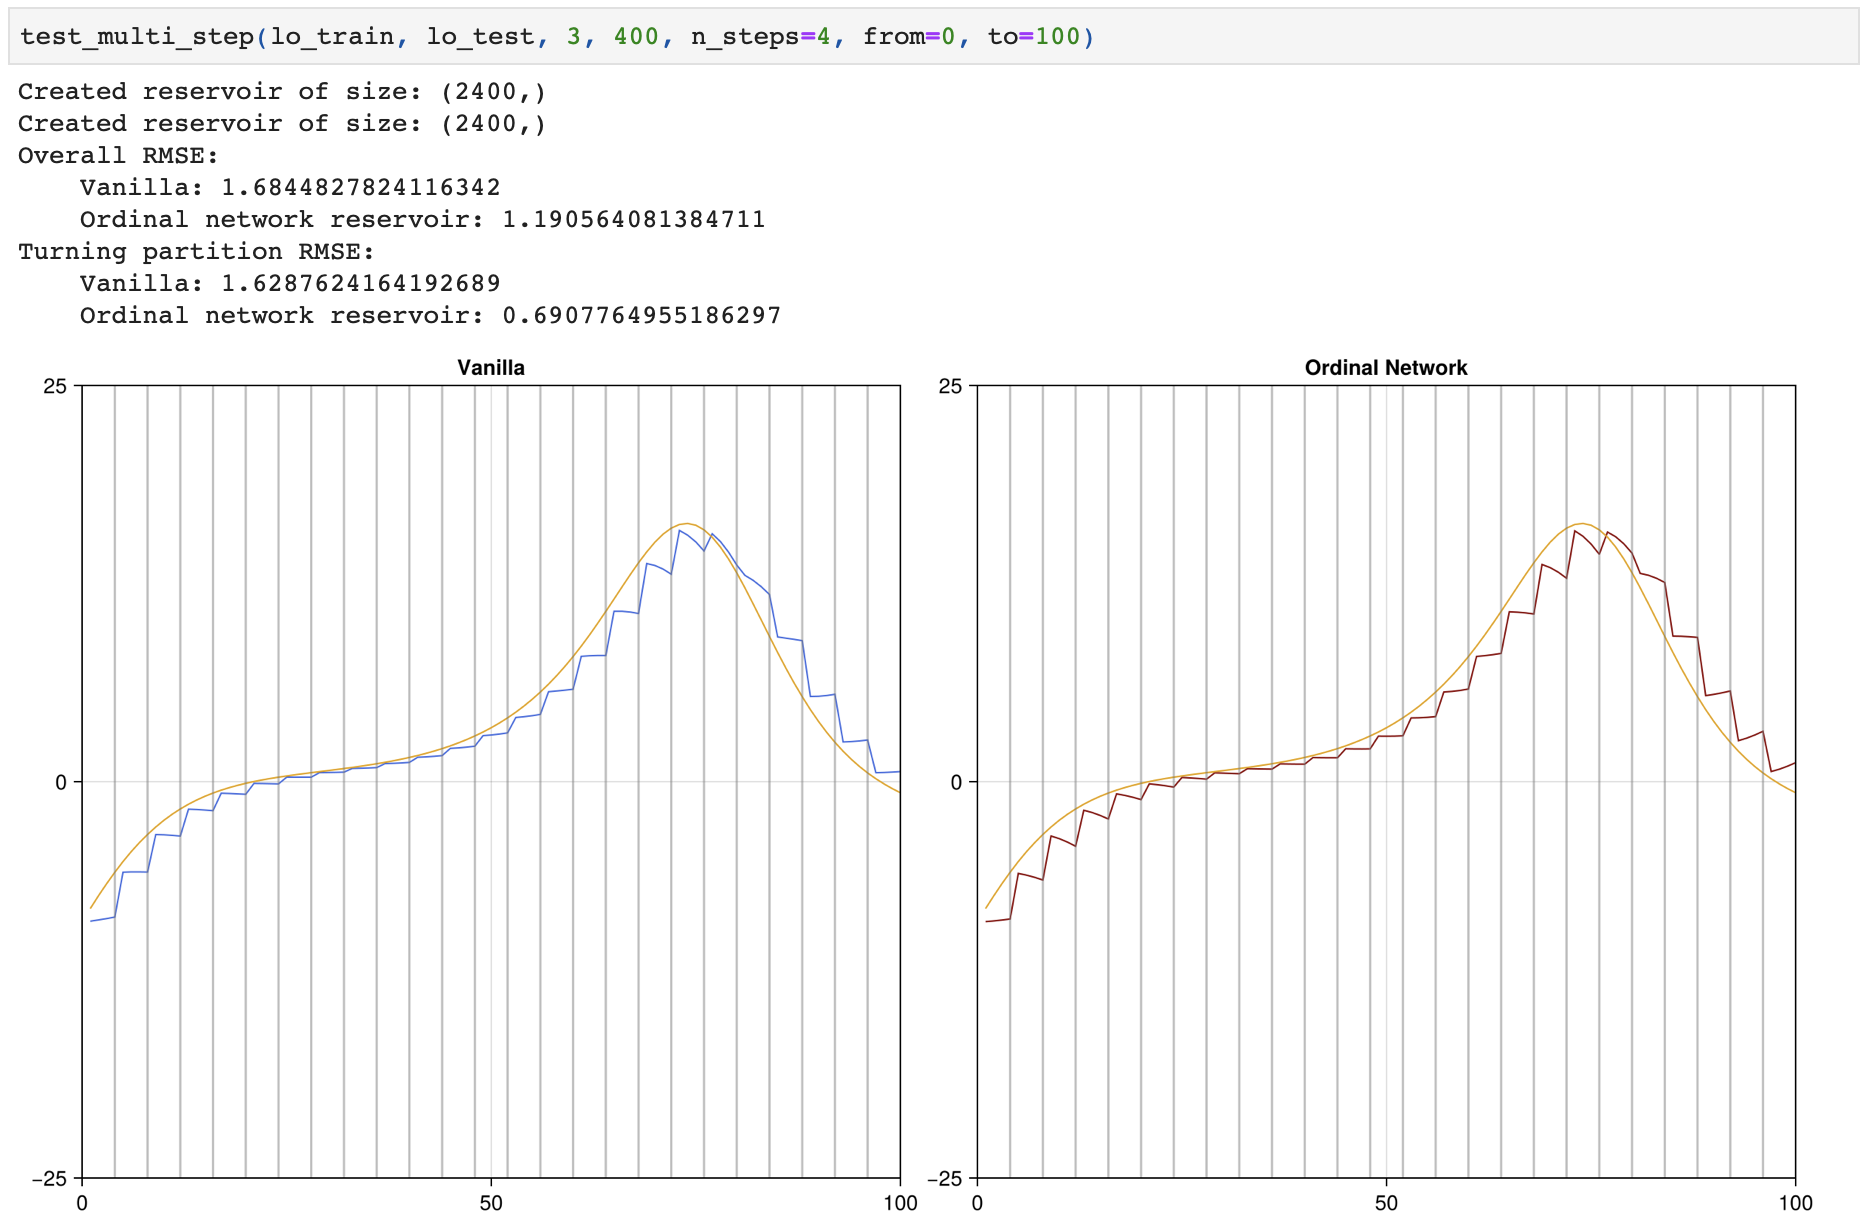
\includegraphics[width=\textwidth]{figure_3.png}
%\end{figure}




Since each run randomly initialises the ESNs, I decided to do a sample of 30 of these, calculate the RMSE for each sample and take the mean of these sample RMSEs. I feel like this is a bit suspect, and that maybe I should take the MSE over all predictions over all samples before taking the squareroot. What do you think?

Anyway then I did this sampling over different lengths of multi-step prediction to create these plots. For each plot, the total k of the ON ESN vs the vanilla ESN are equal.

\newpage

Vanilla ESN: total k = 300

ON ESN: layer k = 50, m = 3, number of partitions/layers = 6

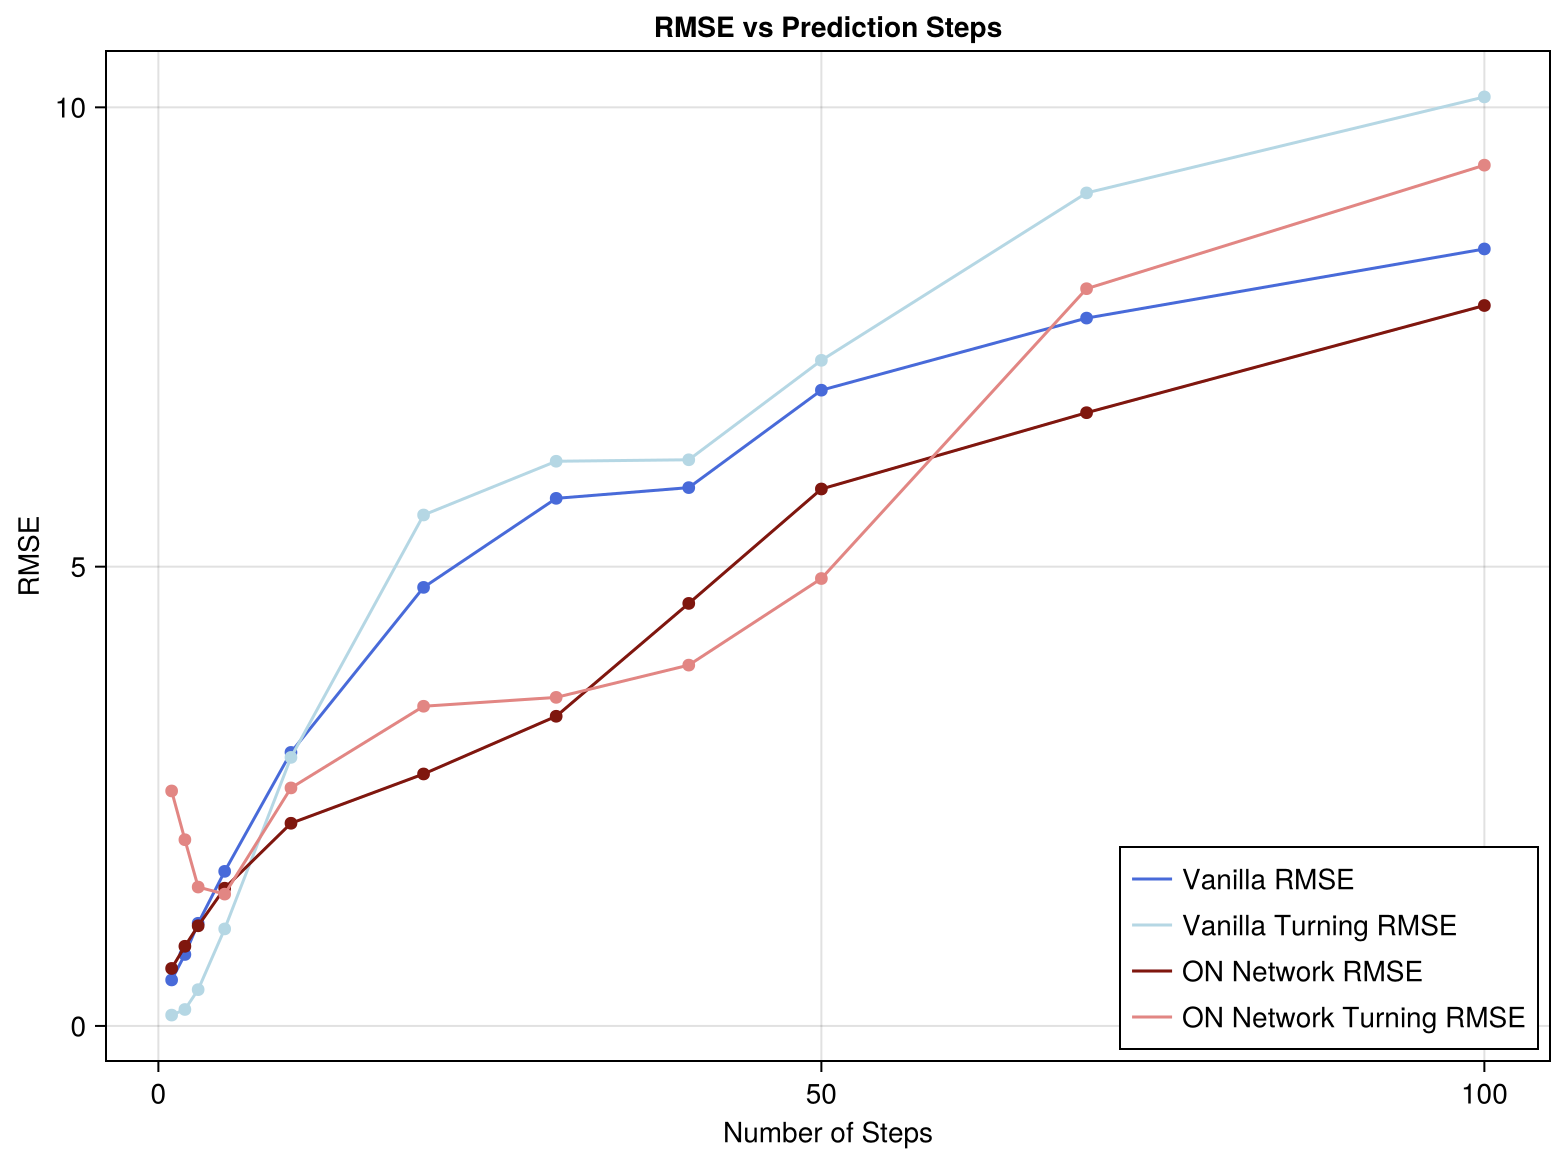
\includegraphics[width=\textwidth]{figure_4.png}


\newpage

Vanilla ESN: total k = 600

ON ESN: layer k = 100, m = 3, number of partitions/layers = 6

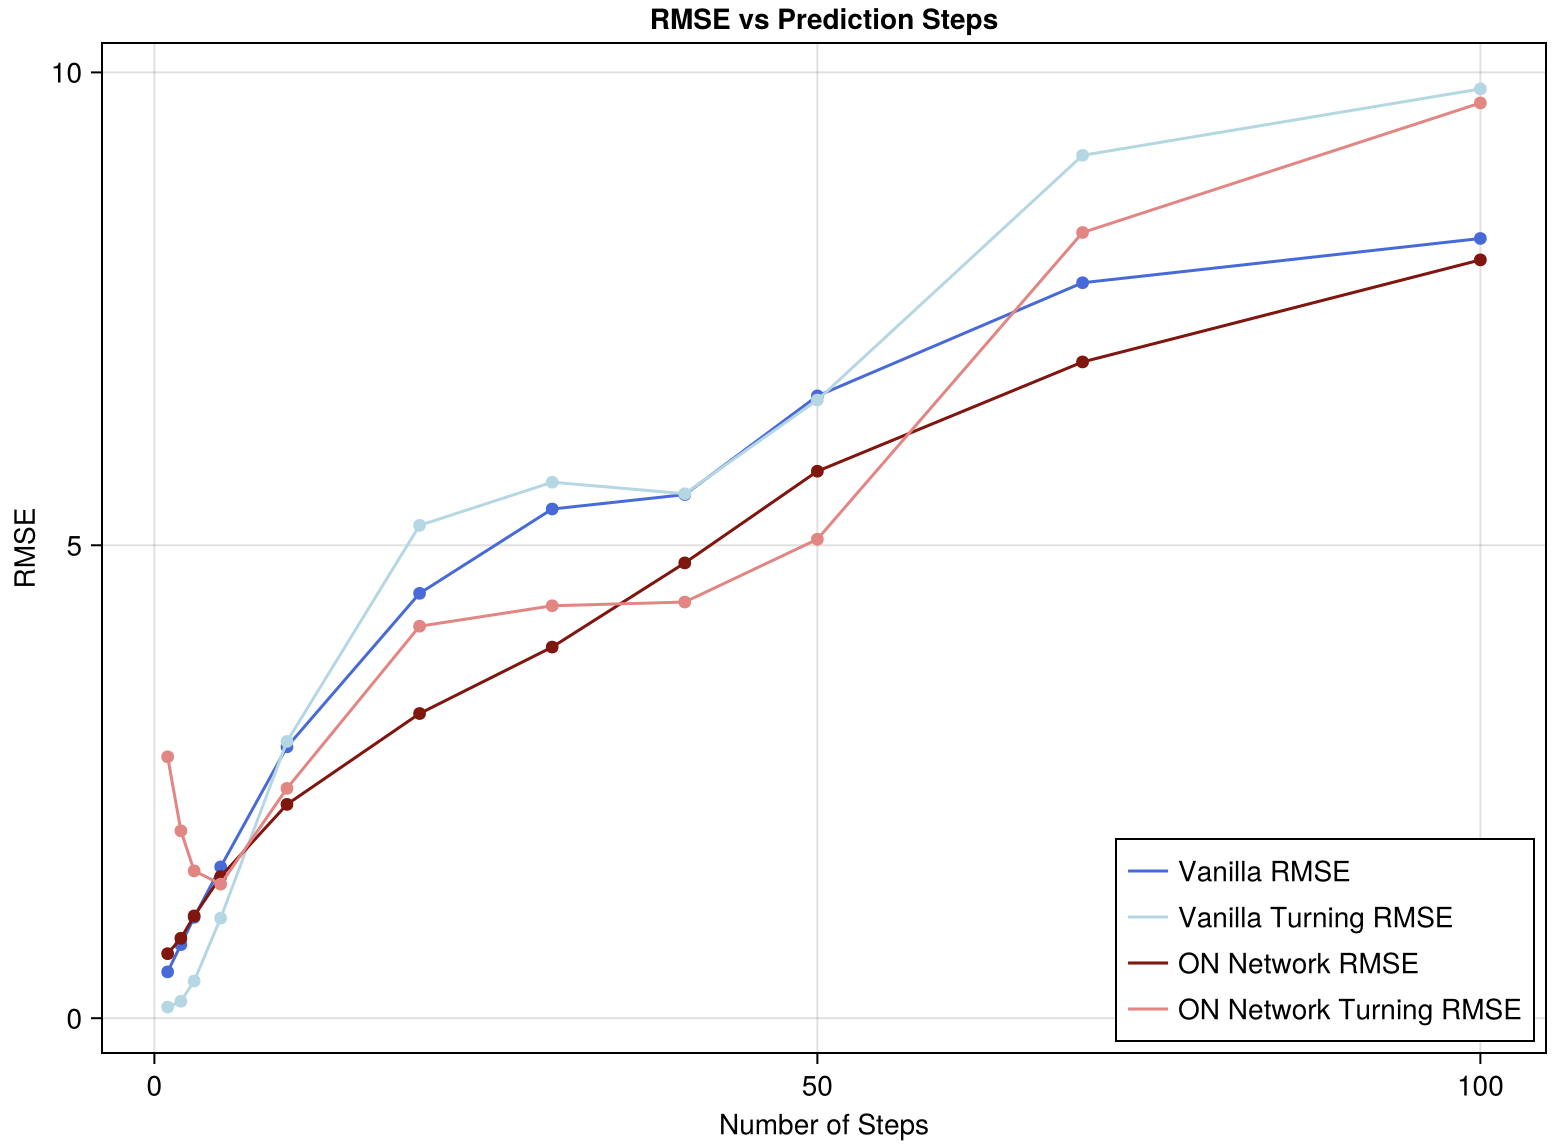
\includegraphics[width=\textwidth]{figure_5.png}


\newpage

Vanilla ESN: total k = 1800

ON ESN: layer k = 300, m = 3, number of partitions/layers = 6

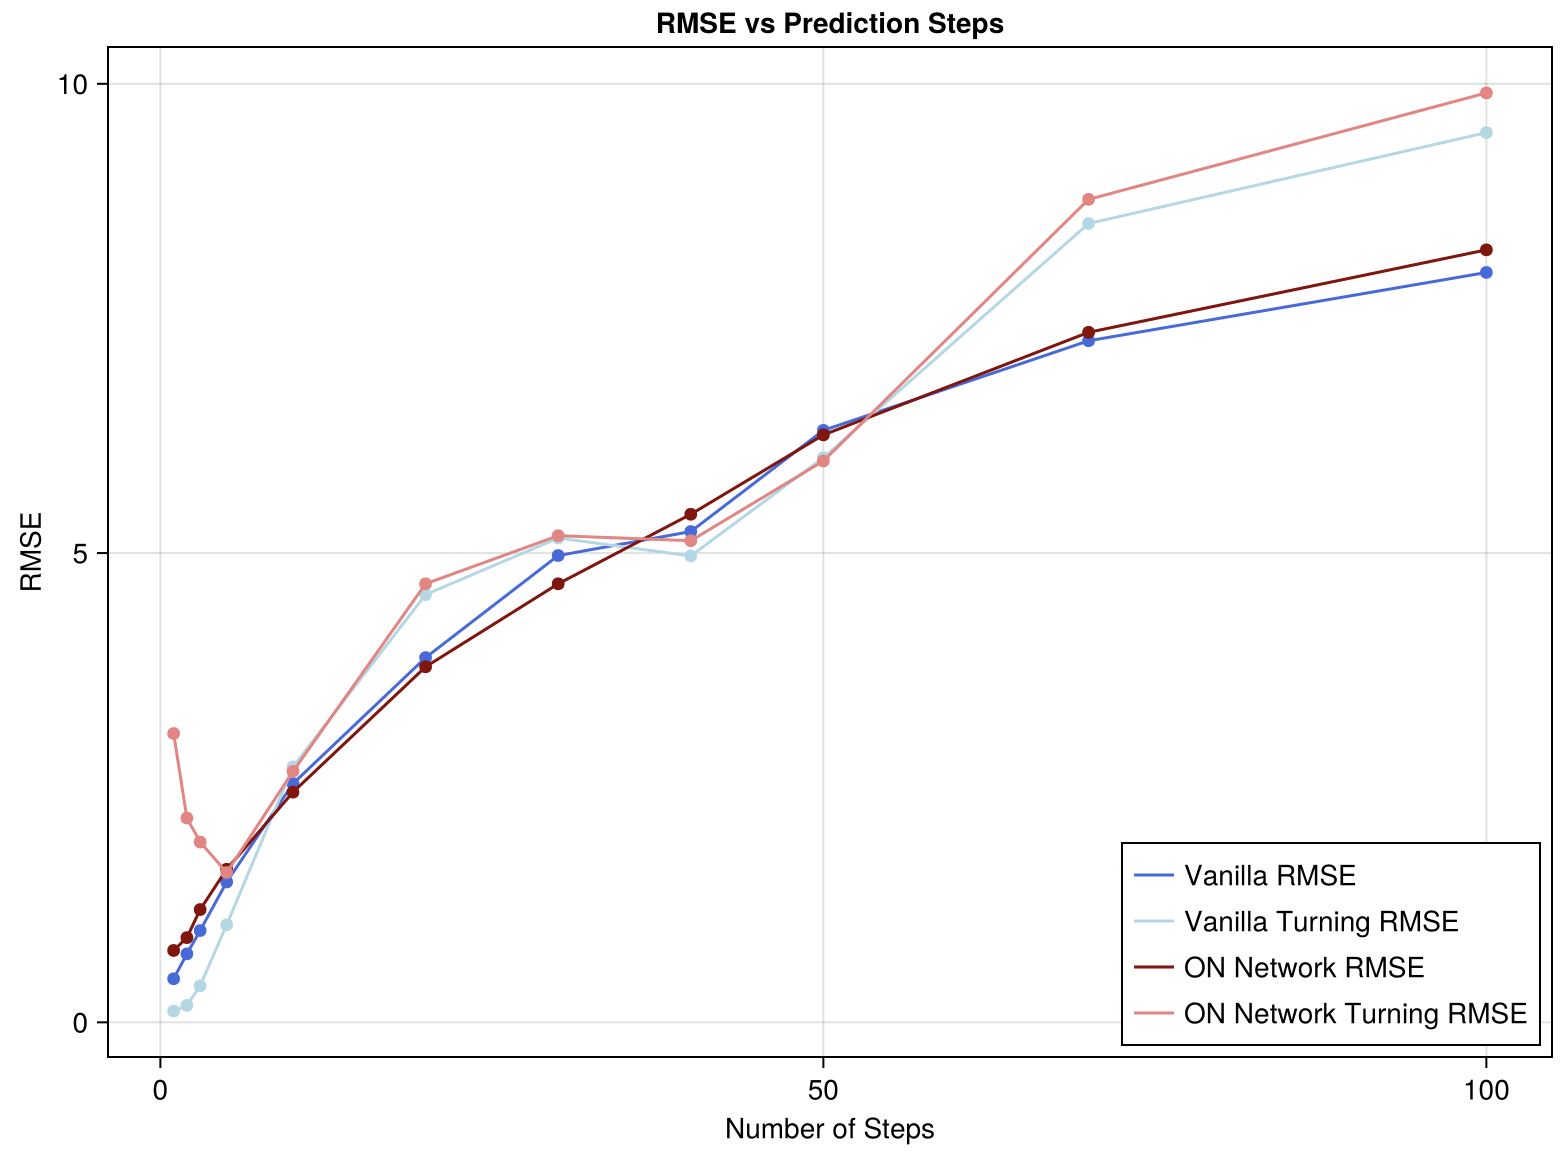
\includegraphics[width=\textwidth]{figure_6.png}


\newpage

Vanilla ESN: total k = 1300

ON ESN: layer k = 100, m= 4, number of partitions/layers = 13

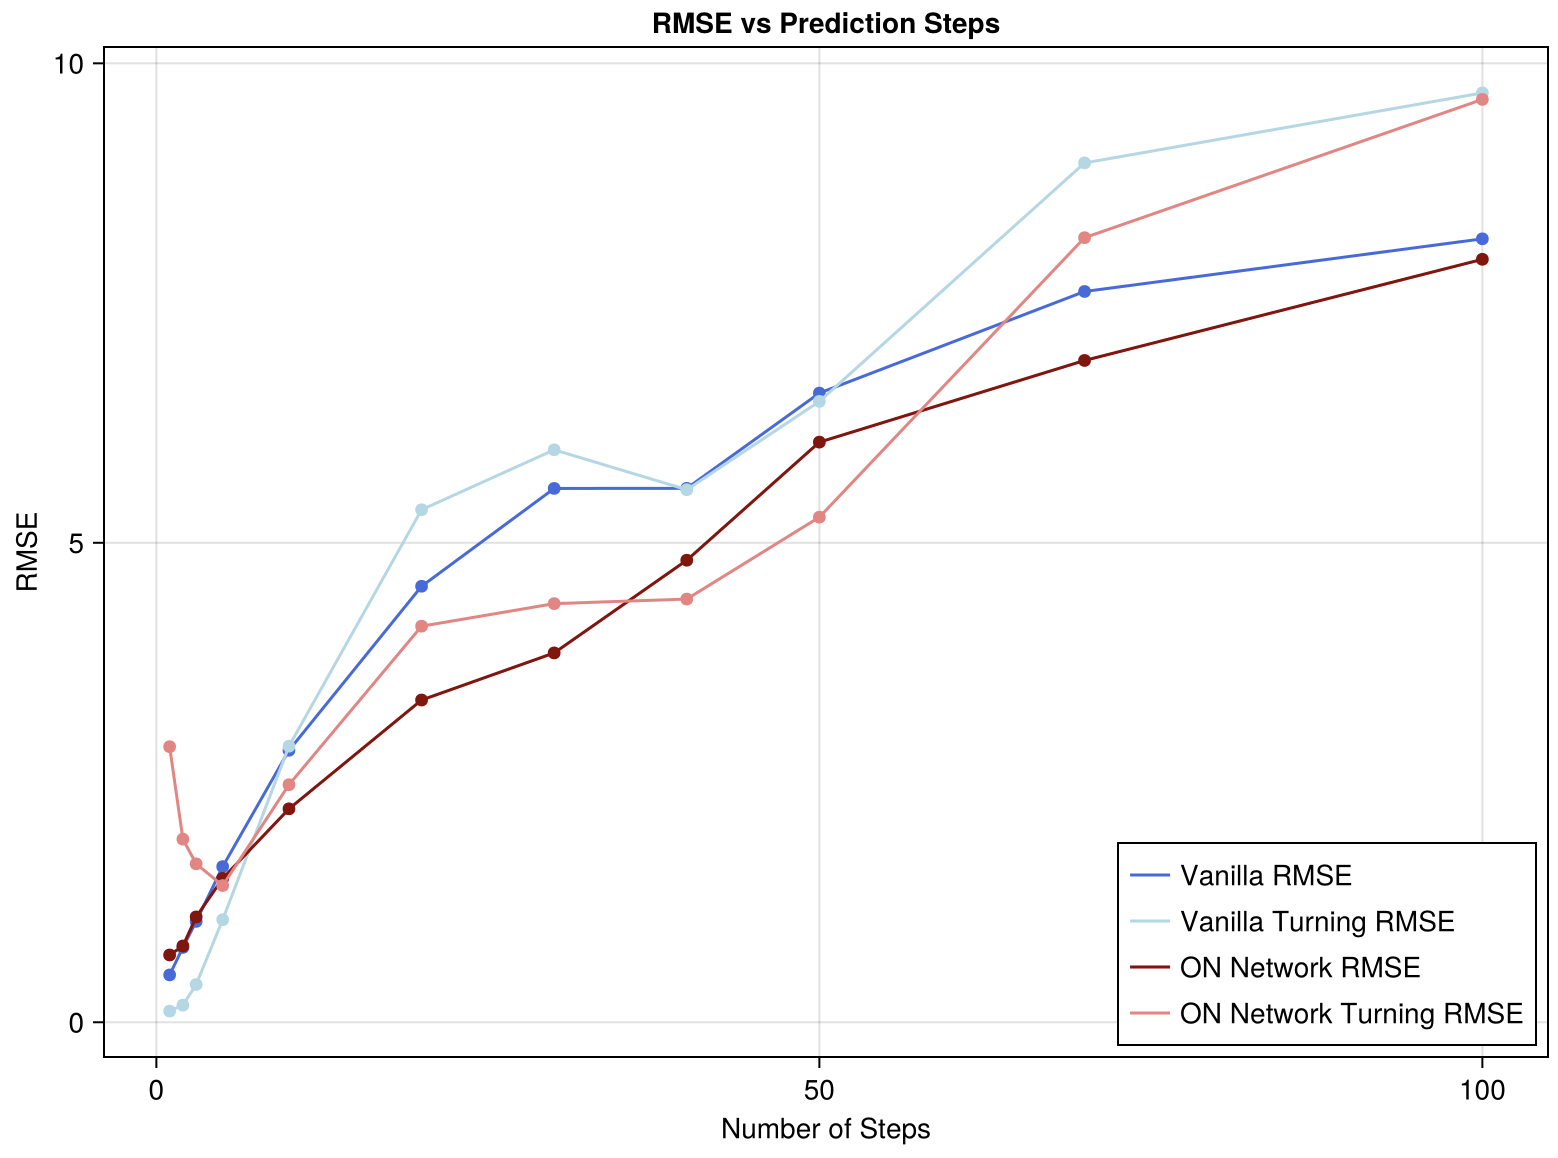
\includegraphics[width=\textwidth]{figure_7.png}


\newpage

Vanilla ESN: total k = 3250

ON ESN: layer k = 250, m= 4, number of partitions/layers = 13

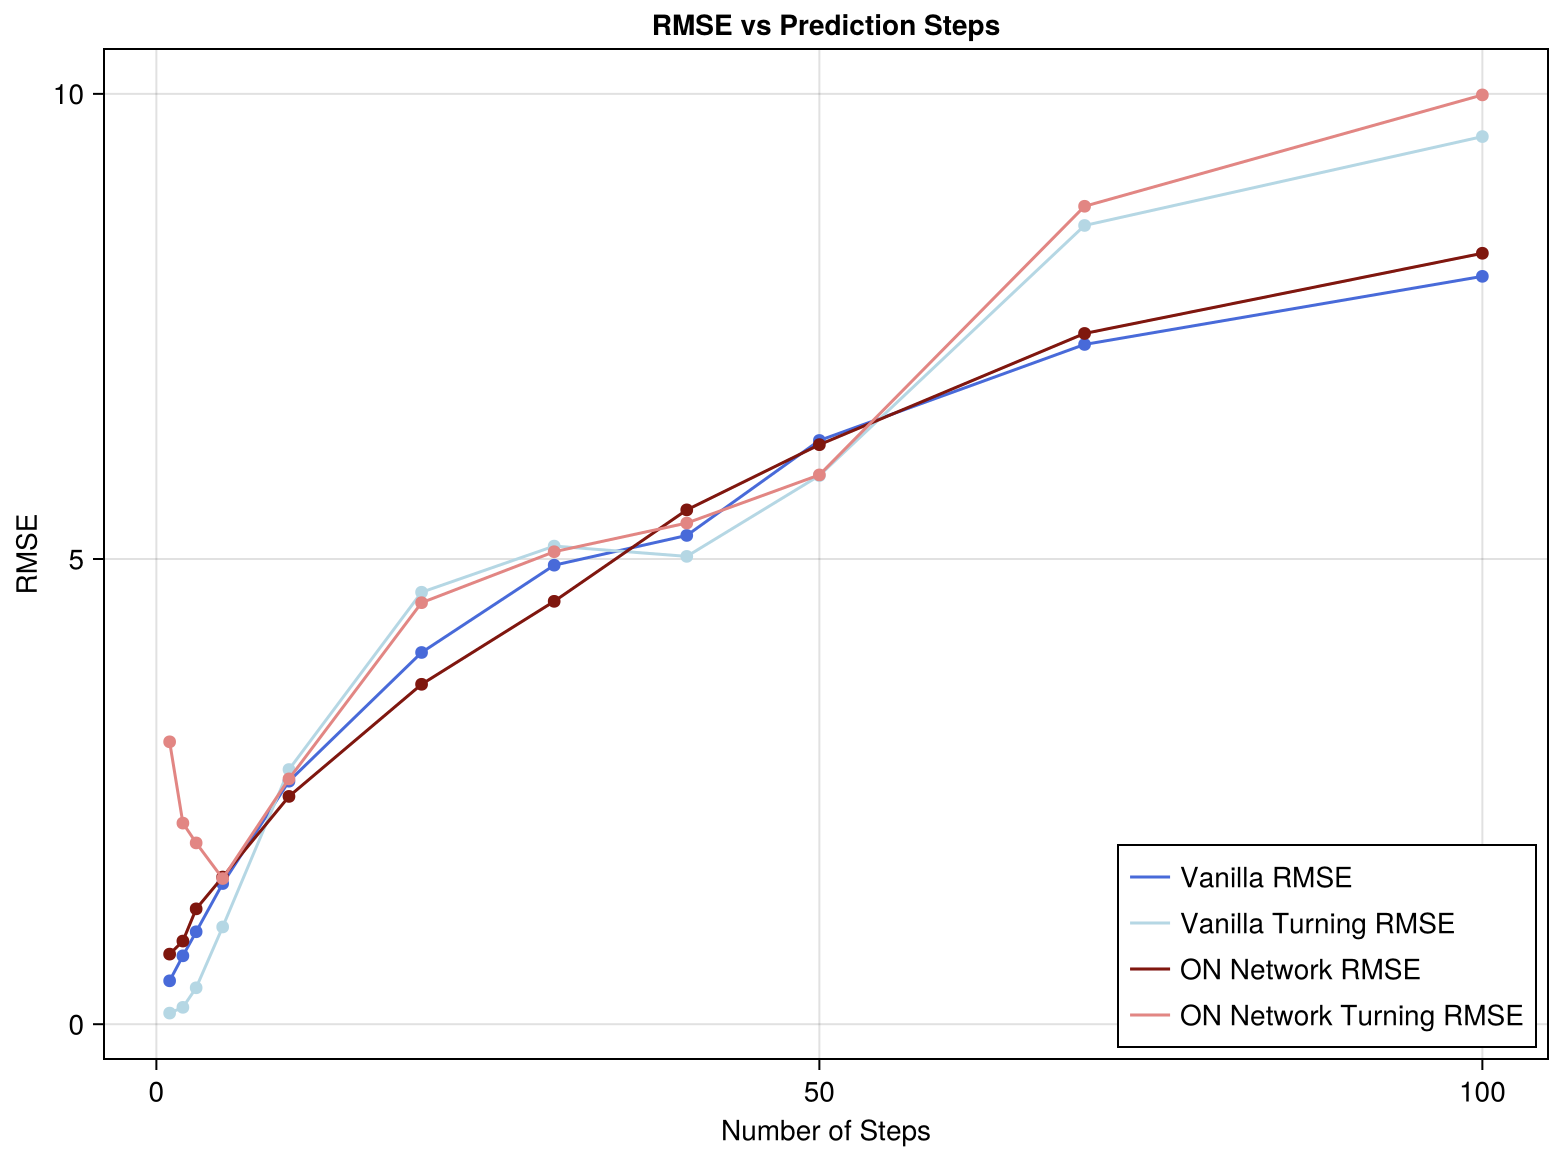
\includegraphics[width=\textwidth]{figure_8.png}


As you can see the ON ESN performs worse than the Vanilla ESN for no. steps predicted below ~5 but appears to perform better above ~5 step predicted. However, this effect seems to wash out for higher values of k (size of reservoir).



\textbf{Note: I spent a while making a little testing framework to make it easier to parse parameters for comparison. Most of the code is now in scripts, with notebooks just to show the graphs.}



\section{Readout Masking}

\textbf{Hypothesis}: masking all layers other than the active layer (corresponding to the current ordinal partition) before performing the readout (i.e. just before doing predictions = states*R) will improve prediction.

\textbf{Findings}:

Initially, it looked as though it didn't make a difference whether or not the readout was masked, based on single step predictions. I came to this opinion just from running the single step predictions a few times and seeing that the RMSE was approximately the same.

But once I implemented the multi-step predictions and the associated error charts, it looks as though readout masking makes the prediction worse for longer predictions. Here is the RMSE for the ON ESN \textbf{with} readout masking vs the vanilla ESN:

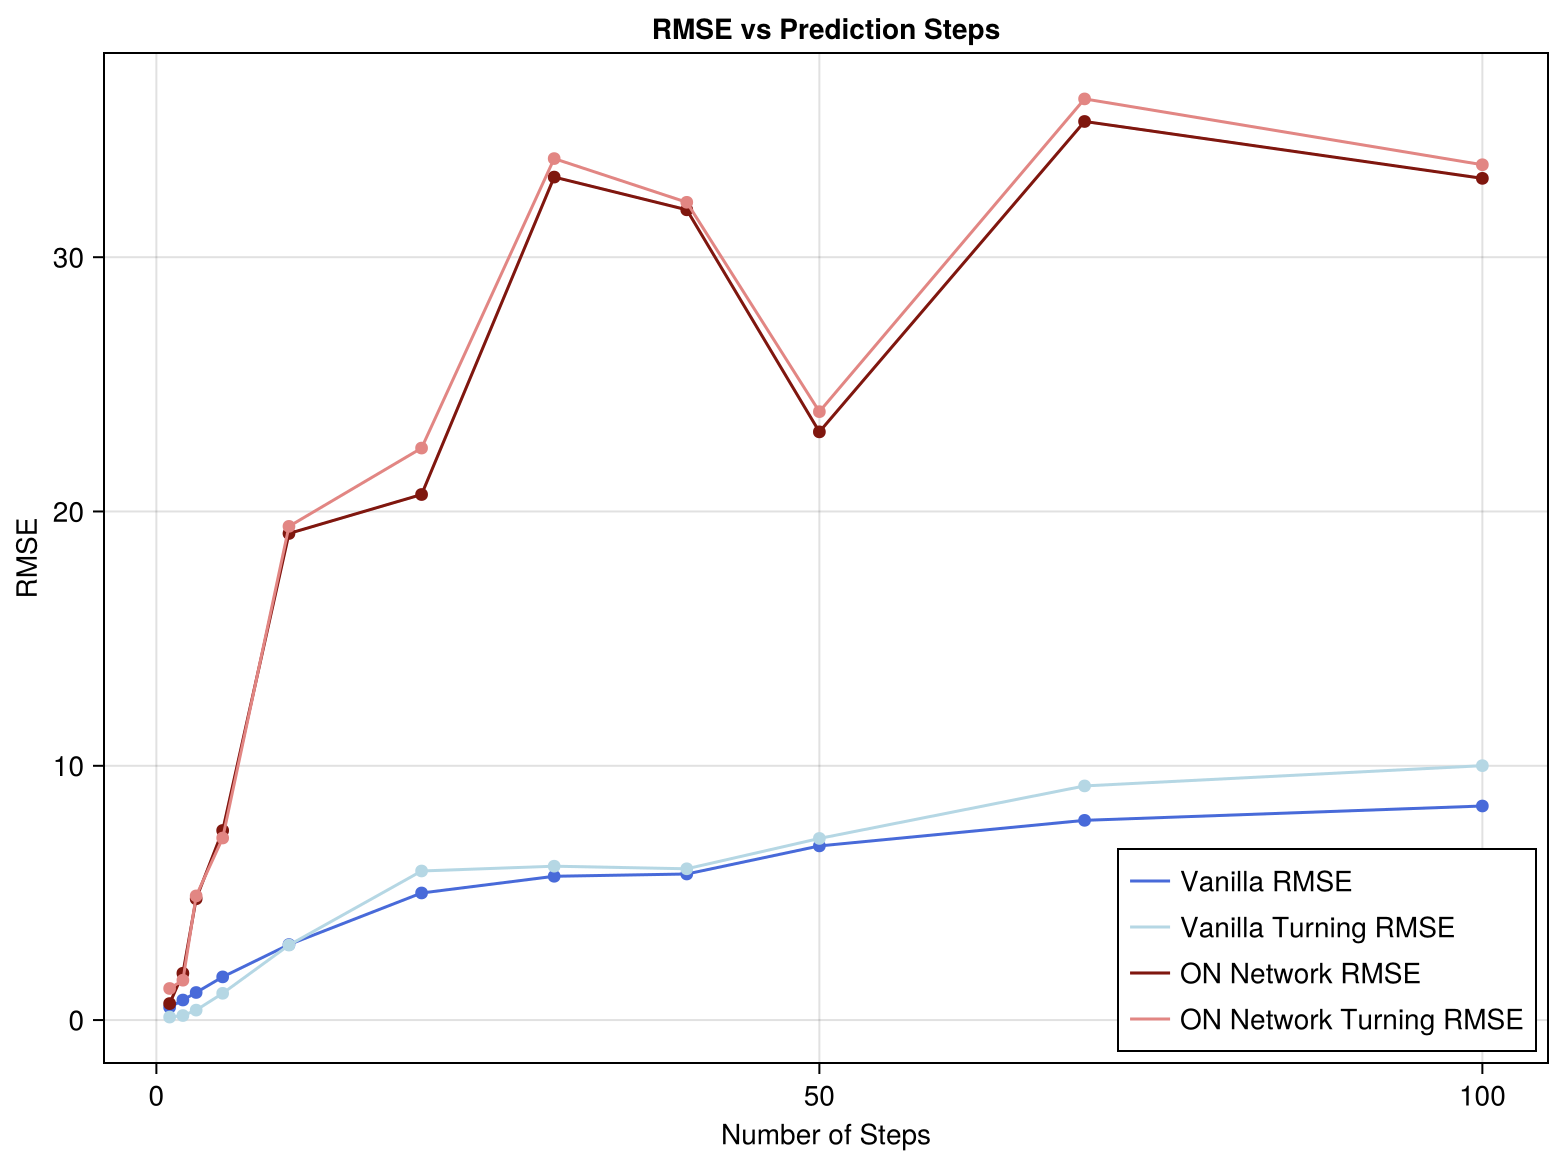
\includegraphics[width=\textwidth]{figure_9.png}


Meanwhile, here is the RMSE for the ON ESN \textbf{without} readout masking vs the vanilla ESN:

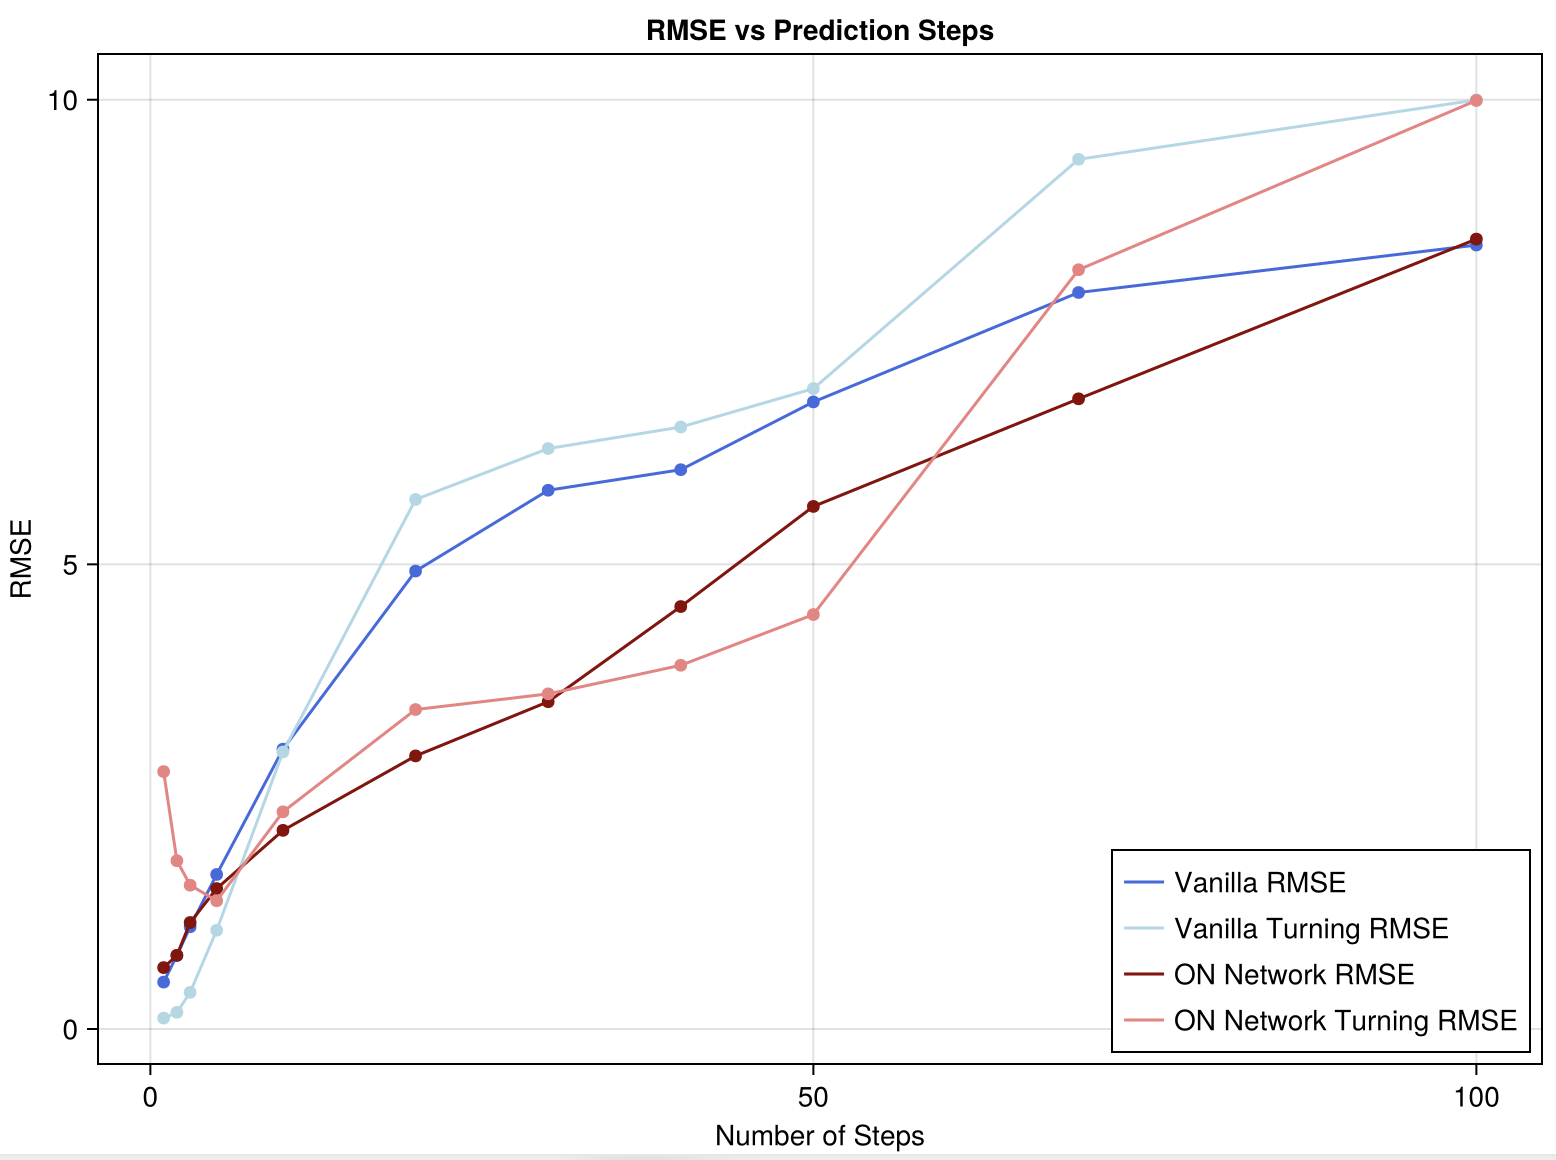
\includegraphics[width=\textwidth]{figure_10.png}


Interestingly, at a lower number of step (i.e. less than ~5) the ON ESN \textbf{with} readout masking looks like it doesn't suffer from the high turning partition RMSE that the ON ESN \textbf{without} readout masking does. Not sure why that would be.



\section{Stochastic ON ESN}

\textbf{Hypothesis}: the predictions will improve if we stochastically choose one other layer for each layer to be connected to based on the transition probabilities of the ON, while masking all other connections.

\textbf{Results}:

The stochastic ON ESN appears to perform well. In this case (see below) it had a lower RMSE.

Left: vanilla ESN with reservoir size 600

Right: Stochastic ON ESN with layer size 100 and 6 layers (given an m=3 to create partitions) - total size 600

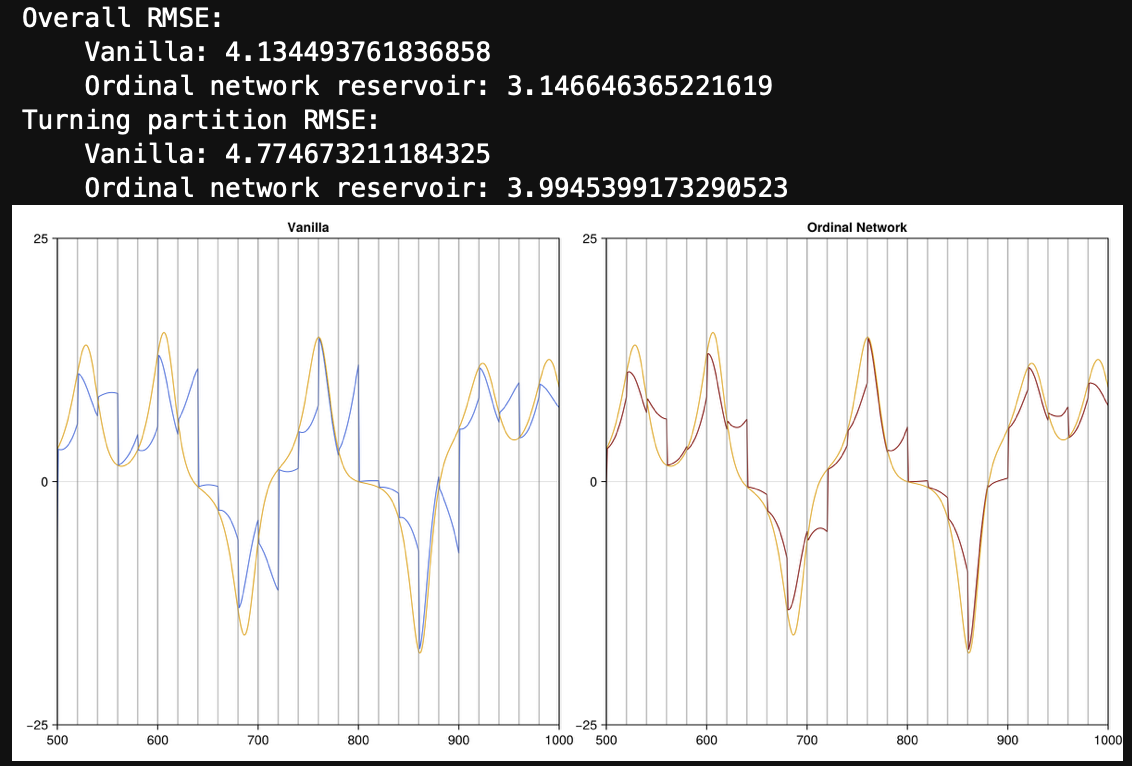
\includegraphics[width=\textwidth]{figure_11.png}


\newpage

So far I have done one thorough test like those above. Here are the results so far for the stochastic ON ESN:

ON ESN: m = 3, layer k = 50, number of partitions/layers = 6

Vanilla ESN: k = 300

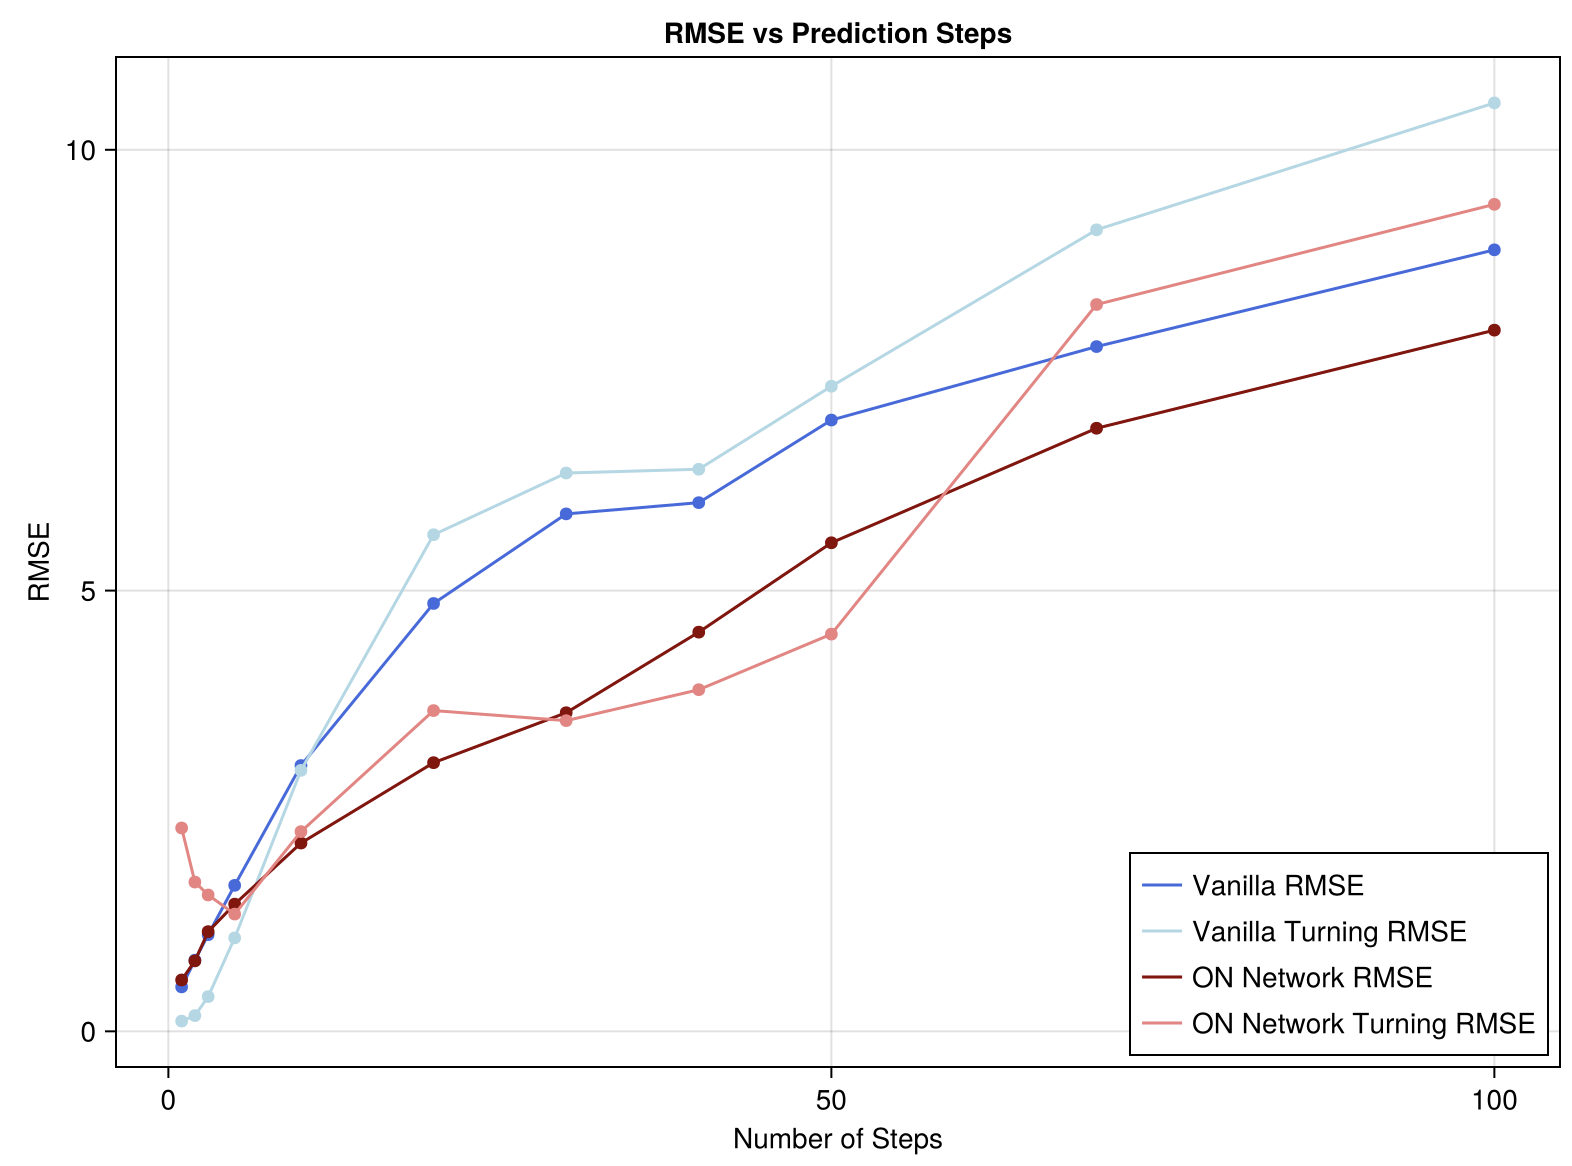
\includegraphics[width=\textwidth]{figure_12.png}

\newpage

Compared to the non-stochastic ON ESN with the same settings:

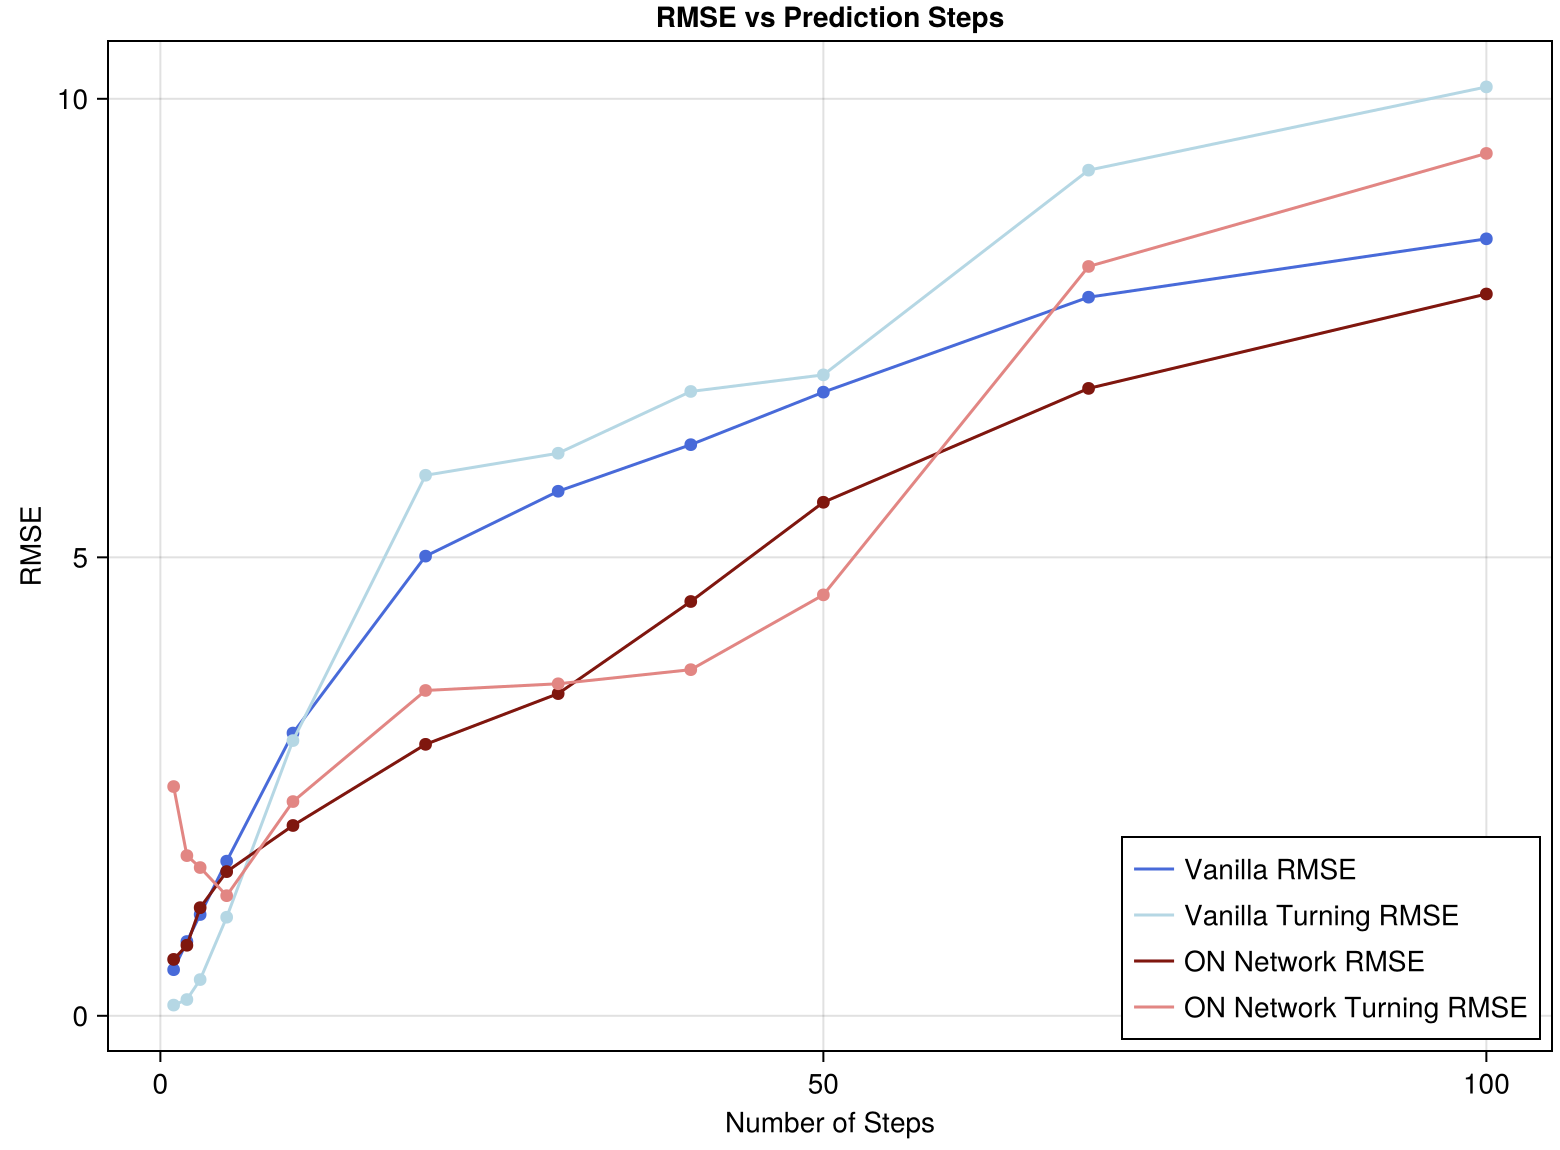
\includegraphics[width=\textwidth]{figure_13.png}



I'm pretty shocked that the results are very similar to the non-stochastic ON ESN. I've checked thoroughly for errors but haven't found anything yet - maybe I will tomorrow lol. I'm almost expecting to. Otherwise it's pretty amazing that they'd be so similar. It could be explained by the fact that the time step for the Lorenz simulation is small at 0.01, so the stochastic switching of layer connections average out to be pretty similar to the deterministic layer connections. Perhaps I will compare the pair at a longer time step.


\newpage

\section{Next steps}

I'm planning to:

\begin{itemize}
    \item Make thorough multi-trial test for single step predictions, like I have for multi-step predictions.
    \item Keep testing the stochastic ON ESN and comparing it to the deterministic (regular) ON ESN.
    \item Thoroughly test the difference between:
    \begin{itemize}
        \item scaling the layer connections according to the transition probabilities, vs
        \item Having a constant value connection, vs
        \item Randomising the connection, vs
        \item Making it sparsely connected.
    \end{itemize}
    \item Test adding self loops (low priority)
\end{itemize}

Looking forward to hearing your thoughts! As always you can check up on me here:
https://github.com/HectorMorlet/echo-state-networks


%\begin{figure}
%\centering
%\begin{subfigure}{.5\textwidth}
%  \centering
%  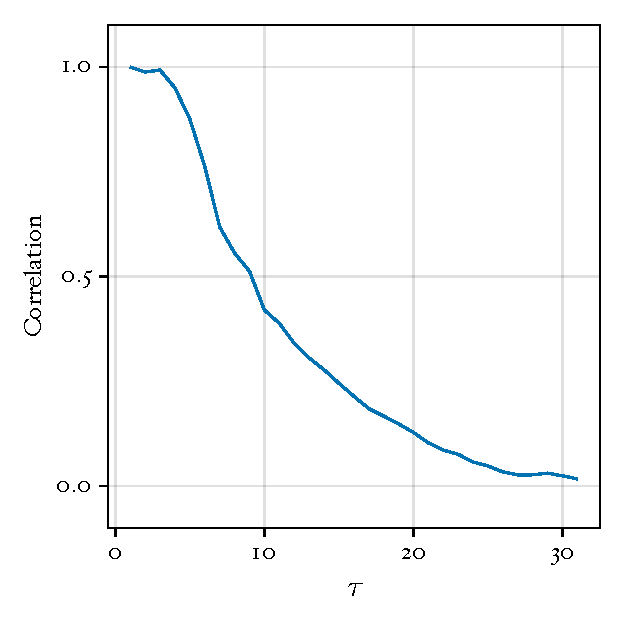
\includegraphics[width=\linewidth]{correlation}
%  \caption{Correlation over $\tau$}
%  \label{fig:correlation}
%\end{subfigure}%
%\begin{subfigure}{.507\textwidth}
%  \centering
%  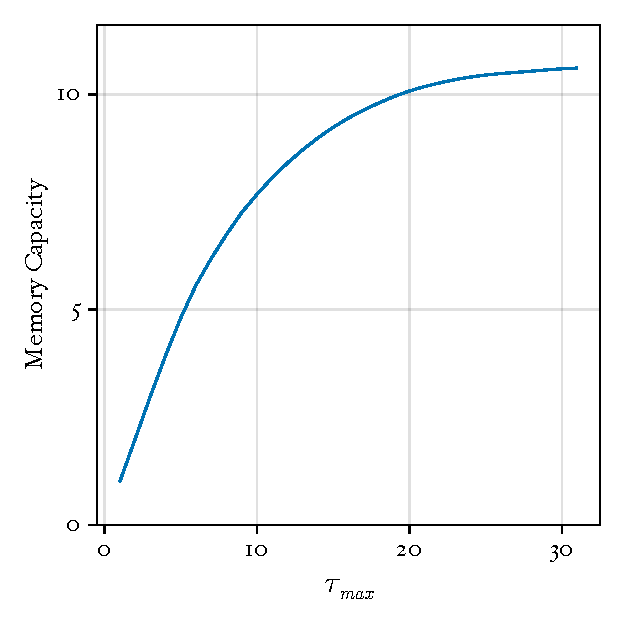
\includegraphics[width=\linewidth]{memory_capacity}
%  \caption{Convergence of memory capacity $MC(\tau_{max})$}
%  \label{fig:memory_capacity}
%\end{subfigure}
%\caption{Measures of correlation and memory capacity over time delay $\tau$ for an example reservoir computer, an Echo %State Network with 100 nodes and $\rho=2$.}
%\end{figure}

\end{document}
